\chapter{Introduction}
\label{cha:introduction}

The isolation of graphene demonstrated that reducing a material to the atomic scale can generate electronic, optical, and quantum properties that differ substantially from those of its bulk form~\cite{novoselov2004electric,geim2007rise}.
Since then, two-dimensional materials have become a major platform in condensed matter physics and materials science.
Reduced dimensionality reshapes the electronic states, enhances the role of surfaces and interfaces, and strengthens the connection between symmetry, bonding, and physical response.
These features allow two-dimensional systems to host properties that are difficult to obtain in conventional three-dimensional crystals.

Beyond graphene, the family of atomically thin materials has expanded to include elemental sheets commonly referred to as Xenes, as well as related light-element compound two-dimensional materials~\cite{butler2013progress,molle2018silicene}.
Light-element Xenes, such as o-\ce{B14} shown in Figure \ref{fig:intro}, and related compounds are especially attractive because their low atomic masses, strong covalent bonding, and flexible bonding environments can produce diverse electronic phases.
Depending on atomic arrangement and chemical modification, these systems may exhibit metallicity, semiconductivity, magnetism, superconductivity, non-trivial topology, and anisotropic optical response.
They therefore provide a compact route for exploring quantum behaviour in ultrathin materials.

\begin{figure}[!htbp]
\centering
    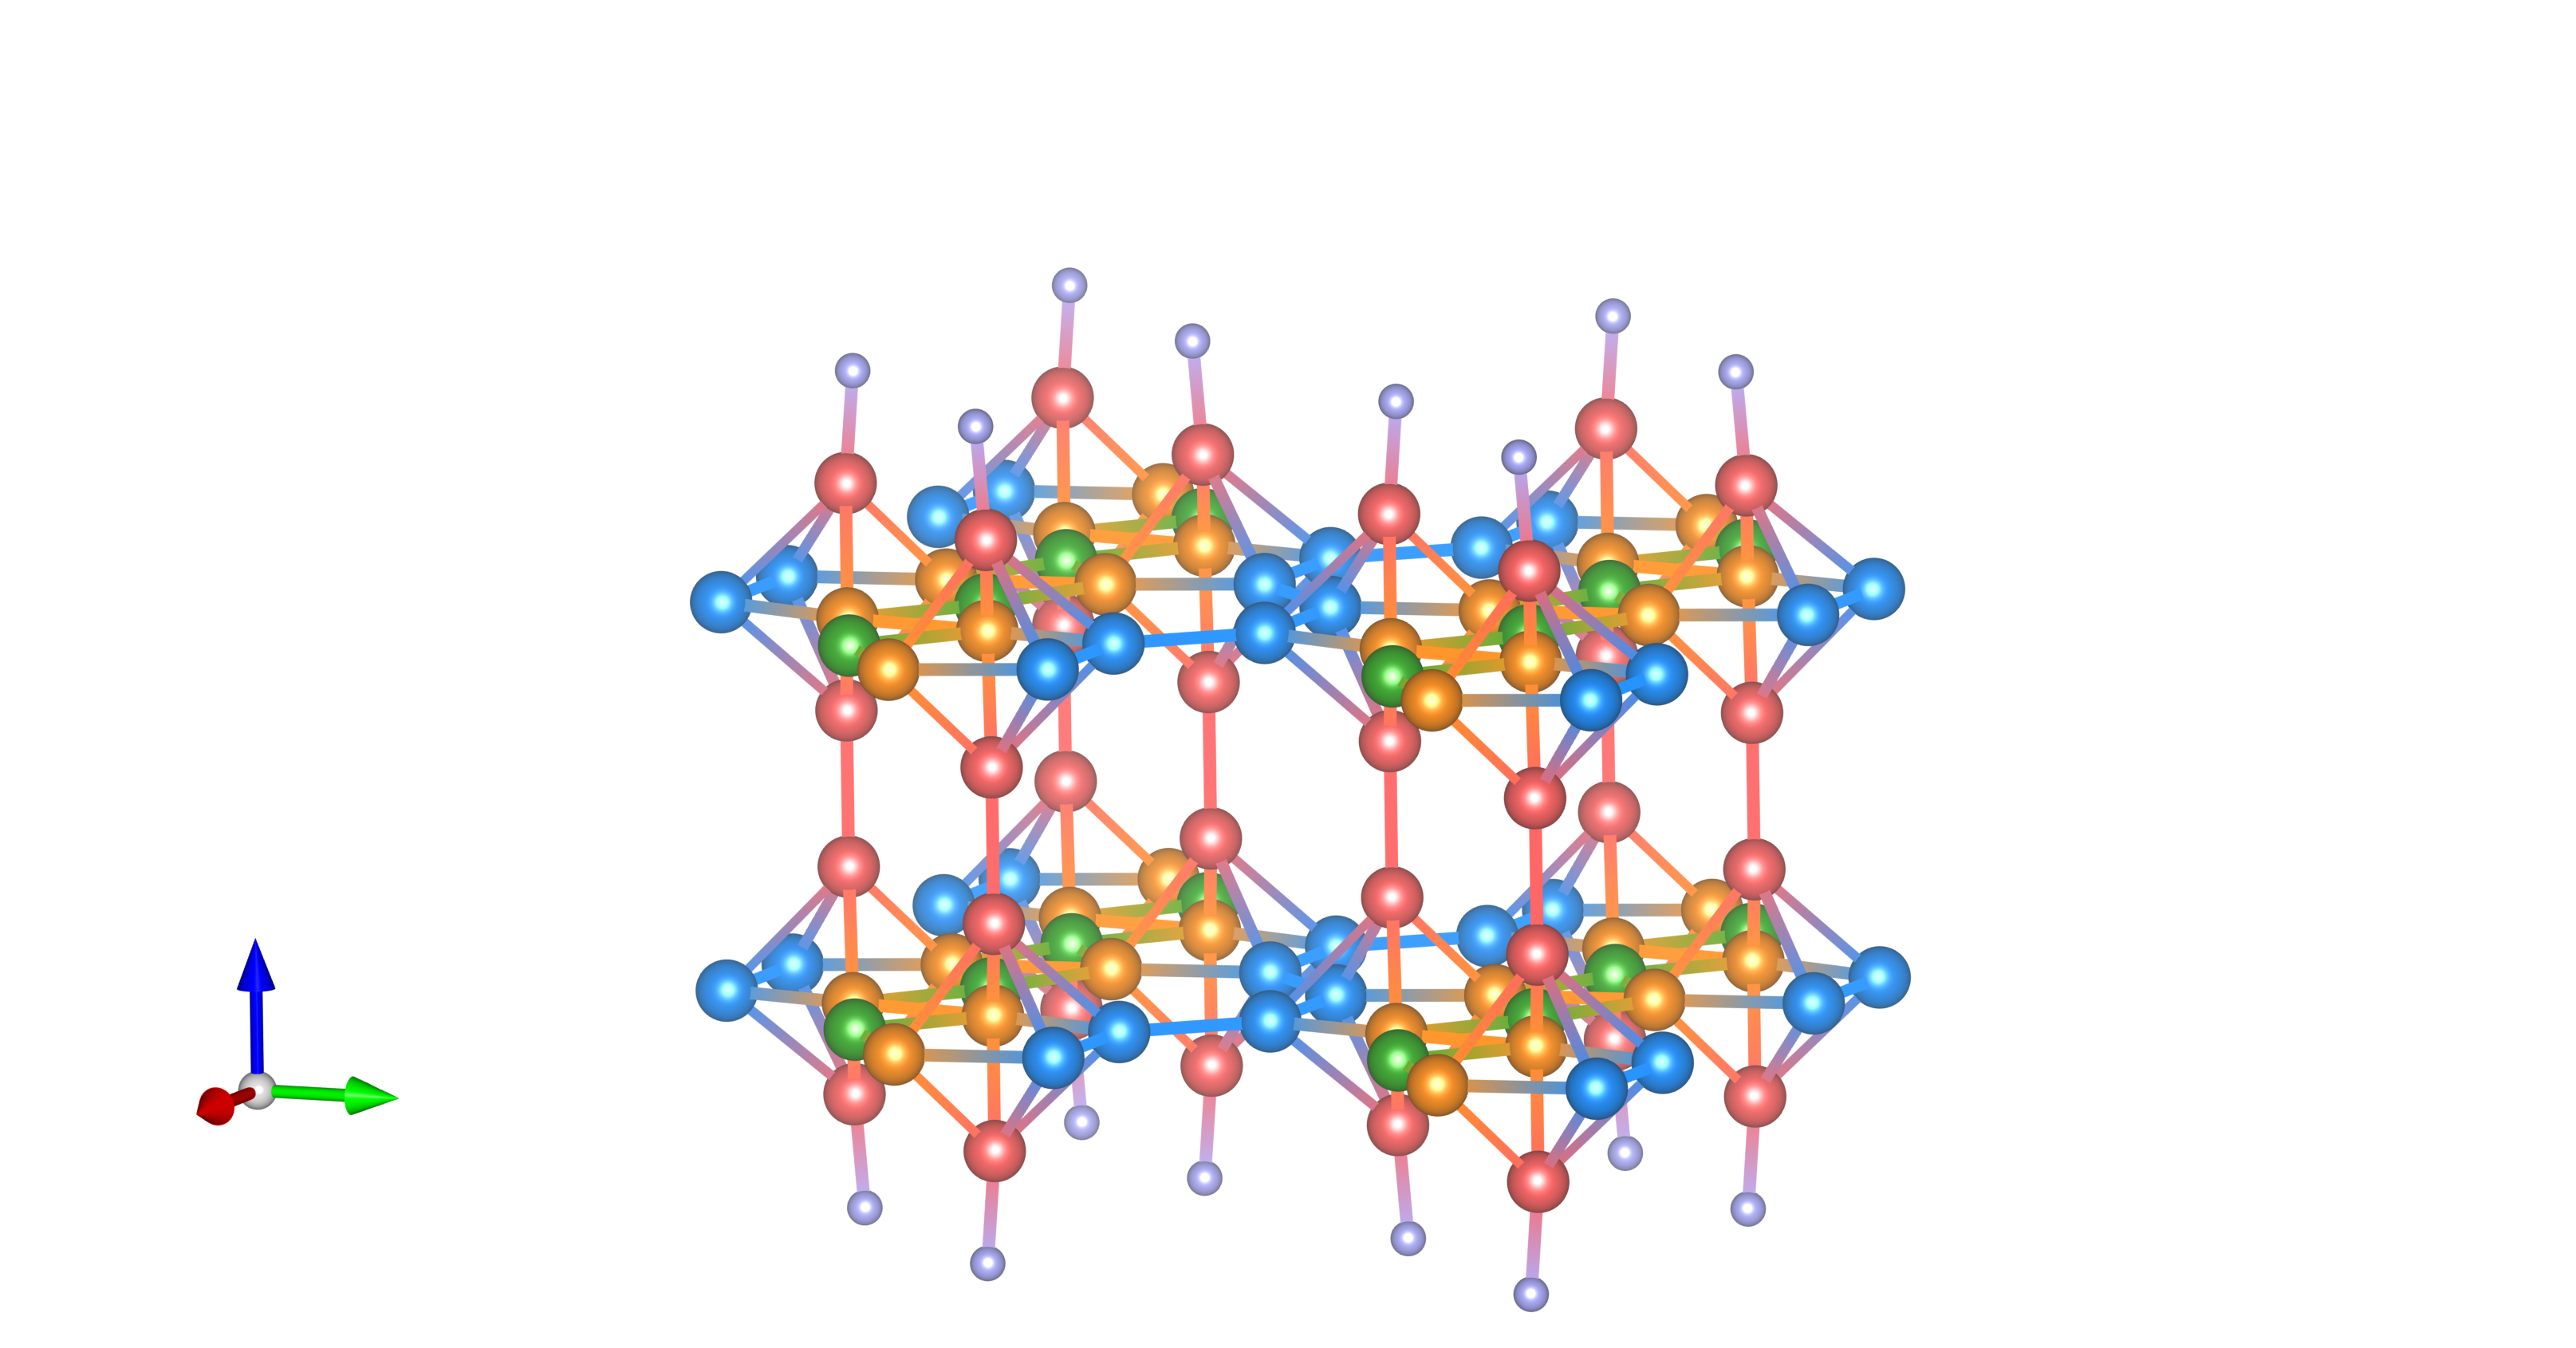
\includegraphics[width=0.6\linewidth]{figures_ch1/intro.png}
\caption{Atomic structure of hydrogen-terminated bilayer \ce{o-B14}. Large coloured spheres represent boron atoms, with different colours denoting crystallographically inequivalent boron sites. Small light-purple spheres represent hydrogen atoms.}
\label{fig:intro}
\end{figure}

Boron-based two-dimensional materials occupy an important position in this landscape.
Unlike carbon, boron is electron deficient, and this electron deficiency favours multicentre bonding and structural diversity.
As a result, boron can form many competing atomic networks with distinct electronic and collective properties.
Boron allotropes and boron-containing compounds therefore provide natural systems for examining how bonding topology controls quantum phenomena.
Beryllium-based two-dimensional materials offer a complementary limit.
Beryllium is the lightest alkaline-earth metal, and its two-dimensional phases remain much less explored than graphene, borophene, and other widely studied xenes.
This makes beryllene a useful platform for testing how reduced dimensionality, hydrogen functionalization, and topology reshape the properties of an elemental light-metal system.

A central challenge in two-dimensional materials research is to tune intrinsic properties for specific physical functions.
Van der Waals heterostructure formation provides one route.
In such systems, different monolayers are stacked through weak interlayer interactions, and the interface can modify electronic states, charge transfer, optical transitions, and collective excitations while preserving important features of the individual layers~\cite{novoselov20162d}.
Surface functionalization provides another route.
Hydrogen adsorption or chemical termination can alter bonding, redistribute electronic states, and change the dielectric response.
These strategies connect atomic-scale design with electronic, optical, superconducting, and topological behaviour.

First-principles calculations provide the practical framework for this connection.
Density functional theory allows us to determine stable structures, electronic bands, densities of states, phonon dispersions, dielectric functions, and derived optical properties from the atomic structure.
In this thesis, we use first-principles calculations to investigate light-element two-dimensional systems based on boron and beryllium.
The central goal is to determine how composition, stacking, bonding topology, reduced dimensionality, and hydrogen functionalization control the electronic structure and optical response.
For selected systems, the analysis also addresses magnetism, superconductivity, and non-trivial topology.

Chapter~\ref{cha:fundamentals_a} introduces the many-body quantum framework behind density functional theory.
The discussion starts from quantum time evolution and the many-body Schrödinger equation, then moves toward the electron density as the central variable.
It introduces the Hohenberg--Kohn theorem, the Kohn--Sham construction, and the practical exchange-correlation approximations used in first-principles calculations.
Chapter~\ref{cha:fundamentals_b} then develops the linear optical response framework used throughout the thesis.
It starts from Maxwell's equations in matter and the constitutive relation, introduces the dielectric tensor and the complex dielectric function, and derives the absorption coefficient, refractive index, extinction coefficient, reflectivity, and energy-loss spectrum from the dielectric response.

The graphene-based heterostructure study in chapter~\ref{cha:project_bilayers} examines van der Waals bilayers formed from graphene, borophene, and two-dimensional boron carbides, namely \ce{BC3} and \ce{B4C3}.
This study asks how combining graphene with different boron-based layers modifies the electronic character and optical response.
The isolated monolayers first provide the reference behaviour.
Graphene shows its semimetallic Dirac electronic structure, borophene is metallic, whereas \ce{BC3} and \ce{B4C3} are indirect-gap semiconductors.
The corresponding bilayers then demonstrate how weak interlayer coupling can tune band structures and dielectric response.
The optical calculations reveal visible-region absorption, plasmonic features, and anisotropic dielectric behaviour.
In particular, Graphene-\ce{B4C3} displays non-negligible off-diagonal dielectric tensor components, indicating possible optically active behaviour associated with reduced symmetry.

The penta-bipyramid boron study in chapter~\ref{cha:project_boron} extends the investigation from engineered heterostructures to intrinsic quantum behaviour in boron allotropes.
This chapter examines bulk \ce{o-B14}, monolayer \ce{o-B14}, bilayer \ce{o-B14}, and the hydrogen-terminated bilayer.
The edge-sharing pentagonal bipyramids in \ce{o-B14} create a distinctive bonding network, and this network allows closely related structures to support different electronic phases.
The calculations show that the two-dimensional forms can host semiconductivity, magnetism, and superconductivity, depending on dimensionality and hydrogen termination.
The same structures also exhibit directional optical response and anisotropic plasmonic modes.
This study therefore demonstrates that atomic-scale bonding topology in boron can control both single-particle electronic properties and collective excitations.

The beryllene study in chapter~\ref{cha:project_beryllene} investigates pristine and hydrogen-functionalized two-dimensional beryllium phases.
The systems include pristine \(\alpha\)-beryllene, \(\beta\)-beryllene, a cubic trilayer beryllene phase, and their hydrogen-functionalized counterparts.
The stability calculations confirm the stability of the previously proposed \(\alpha\)- and \(\beta\)-beryllene phases and identify a dynamically stable cubic trilayer structure.
Hydrogen functionalization substantially changes the electronic structure.
It drives \(\alpha\)-beryllene into a wide-gap semiconducting state, while the hydrogen-functionalized \(\beta\)-based structures retain metallic behaviour.
The dielectric response shows strong anisotropy, visible-to-ultraviolet absorption, modified plasmonic behaviour, and direction-dependent screening.
The topological analysis further shows that pristine \(\alpha\)-beryllene and cubic trilayer beryllene possess non-trivial \(\mathbb{Z}_2\) topology.

Finally, chapter~\ref{cha:conclusion_outlook} summarizes the main findings and presents possible directions for future work.
Across the three materials studies, this thesis demonstrates that light-element xenes and related compounds can host complex quantum and optical behaviour when their atomic structures are organized in low-dimensional forms.
Heterostructure formation, bonding topology, reduced dimensionality, and hydrogen functionalization provide practical routes for tuning electronic structure, dielectric response, plasmonic modes, superconductivity, magnetism, and topology.
